\talkslide{joint-game}{A different paradigm: adversarial games}{Timing: provisional}{AdvGame trains two models in one online loop.}{
% Larger illustration, natively clipped to round its corners; original bytes retained.
\begin{tikzpicture}[remember picture,overlay,
 every node/.style={text=Ink,align=left,inner sep=0pt}]
\begin{scope}[shift={(current page.south west)}]
 \node[anchor=north west,text width=14.7cm,font=\normalsize] at (.65,7.0)
   {Train both agents \textbf{concurrently}};
 \begin{scope}
  \clip[rounded corners=8pt] (2.1,1.9) rectangle (13.9,5.617);
  \node at (8,3.7585) {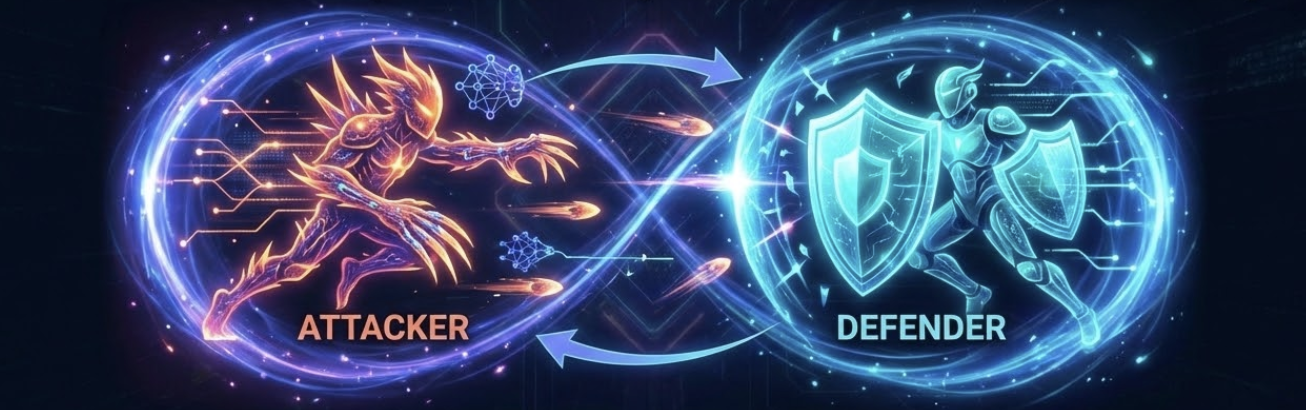
\includegraphics[width=11.8cm]{assets/game-illustration.png}};
 \end{scope}
\end{scope}
\end{tikzpicture}

}
\speak{AdvGame trains two models in one online loop. Each round produces prompts and responses under evolving policies, judges them, and updates both sides. Concurrent adaptation describes this learning process; it does not require every GPU operation or optimizer step to run at exactly the same instant. Each side adapts online to the other's current capabilities. Attack surfaces shift as models change, so a fixed opponent does not capture the whole interaction. We want equilibria reflecting long-run interaction; this is a motivation, not a claim of convergence in neural training.}
